There are two primary phases involved in synthesizing a TrueTime model from an ESMoL model.  First, a new Simulink model containing TrueTime network and kernel blocks must be generated.  These kernel blocks only provide a scheduling and execution framework but do not implement task behaviors themselves.  Therefore, code implementing tasks that will execute within kernel blocks must be supplied.  The second phase synthesizes some ``glue code" that, when compiled with the previously generated functional code, see Section 2 step 3, implements the tasks the TrueTime model will execute.

The first phase, creating the new Simulink model, is itself a two step process since, due to available Matlab APIs, it is easier to synthesize an M-file script, which in turn generates a Simulink model, than it is to generate a Simulink model directly.  Once generated, the M-file script is run and a new Simulink model is created with the appropriate configuration of blocks.  A one-to-one correspondence exists between ESMoL nodes and buses and TrueTime kernels and networks respectively.  The original Simulink model's plant and reference signal blocks must also be part of the new model.  Fig. \ref{fig:truetime_model} shows the resulting Simulink model generated from the M-file script.
\begin{figure}[ht]
\centering
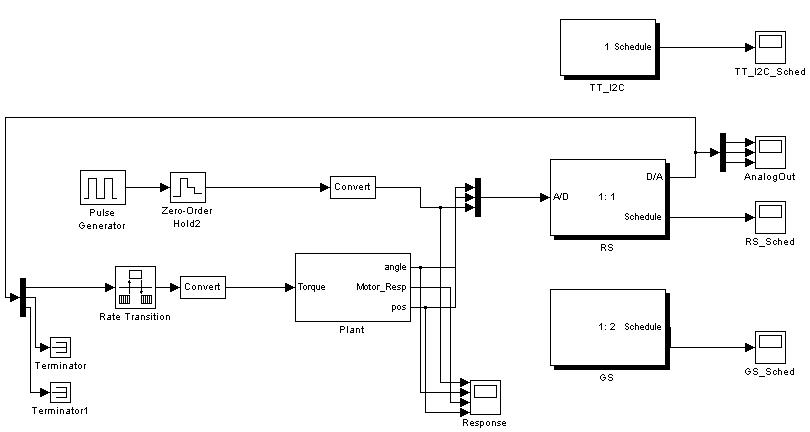
\includegraphics[width=\columnwidth]{figures/truetime.jpg}
    \caption{Synthesized TrueTime model of the quad integrator system}
    \label{fig:truetime_model}
\end{figure}
TrueTime kernels interact with the rest of the Simulink model via ``analog'' inputs and outputs.  Interactions directly between kernels are communicated using the TrueTime network block.  In our example, analog inputs are generated by the ADC and SerialIn blocks and outputs are sent to the SerialOut block, as seen in Fig. \ref{fig:platform}.  The number and ordering of analog signals must be derived from the sensor and actuator messages defined in the ESMoL deployment configuration, as seen in Fig. \ref{fig:deployment}.  Other kernel parameters such as the node number (for network identification) and initial local clock values are similarly derived from the ESMoL model.

The TrueTime network block also must be configured, but does not require any additional code for proper execution.  TrueTime supports a range of networks types: CSMA, Round Robin, FDMA, TDMA, Switched Ethernet, FlexRay, and PROFINET.  Each of these network types must be configured with bus speed, frame size, loss probability, etc.  In our example, a TDMA network block is generated and its properties are configured according to the bus information in the ESMoL model.  A TDMA network was chosen since it implements TTA-like time-based bus access and its timing behavior most resembles that of our $I^{2}C$ bus.

The second phase of creating a TrueTime model is to synthesized the layer of glue code that binds the functional code to the TrueTime run-time.  TrueTime is able to compile and link with either M-file or C/C++ code for task implementations.  In ESMoL both representations of tasks are available, M-file from the original imported controller model, and C-code from the synthesized functional code.  We have chosen to leverage the C functional code since it is identical to the code that will eventually be utilized in a fully deployed control system application.

It is the glue code that implements the semantics of a time-triggered architecture on top of the TrueTime primitives.  TrueTime kernels support both periodic and sporadic execution of tasks.  Neither of these provide the exact timing semantics desired for TTA as they are deadline or period driven and are not guaranteed to begin execution at a specific time.  Given a static TTA execution schedule, tasks should begin execution at their scheduled times.  This requirement necessitates a custom execution scheduler be built on top of the TrueTime scheduler.  This is analogous to implementing a TTA virtual machine on top of a host OS, as discussed in \cite{pvknks_09}.
\begin{figure}[ht]
\centering
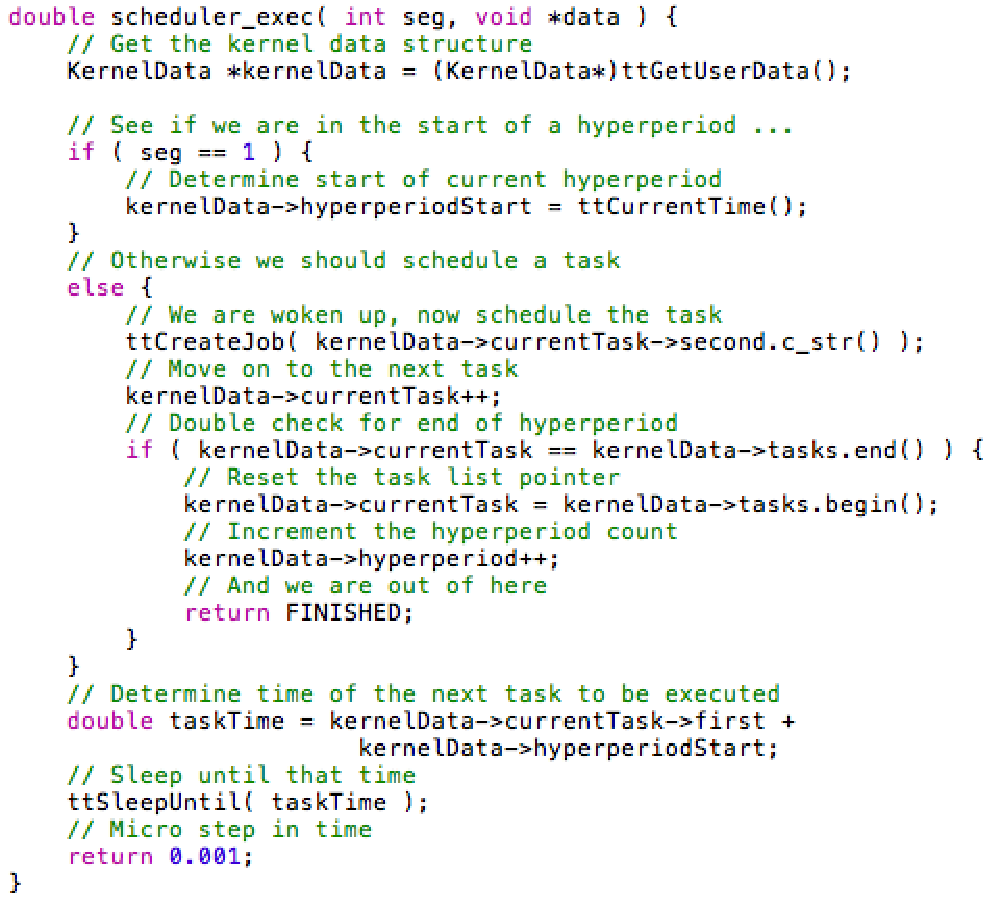
\includegraphics[width=\columnwidth]{figures/scheduler.pdf}
    \caption{Online TTA-based scheduler embedded within each TrueTime kernel}
    \label{fig:scheduler}
\end{figure}
The scheduler used within an ESMoL TTA-based TrueTime model is shown in Fig. \ref{fig:scheduler}.  Our scheduler is implemented as a high-priority periodic task and is scheduled for execution at the beginning of every hyperperiod. TrueTime structures task execution into ``segments''.  A TrueTime task can execute in one or more segments, each of which consumes some finite amount of simulation-clock time.  At the end of each segment the task returns control to the TrueTime scheduler and informs TrueTime of its execution duration via a returned double value.  Any data that must persist between segments or executions must be stored and retrieved in ``UserData'' via TrueTime access functions.

Segment 1 in our scheduler corresponds to the first segment of each execution, and thus the beginning of each hyperperiod.  Our scheduler maintains a sorted map of start times to ESMoL tasks and a pointer that points to the next task to be executed according to this schedule.  During segment 1 the first ESMoL task for the hyperperiod is found and its absolute start time calculated.  The scheduler then sleeps until this time is reached.

When the time has arrived for an ESMoL task to be executed our scheduler should be awoken from sleep by TrueTime.  This corresponds to any segment greater than 1.  ESMoL tasks are implemented as sporadic TrueTime tasks that have a priority lower than our scheduler task.  Our scheduler executes an ESMoL task by scheduling it for execution in TrueTime using the $ttCreateJob()$ function.  Since TrueTime is set to use a priority based scheduling scheme, and no other tasks besides our scheduler are active, as soon as our scheduler ends its segment this new job will execute.  This approach ensures that an ESMoL task starts execution at its statically scheduled time.  ESMoL tasks interact with the TrueTime runtime using segments also.
\begin{figure}[htb]
\centering
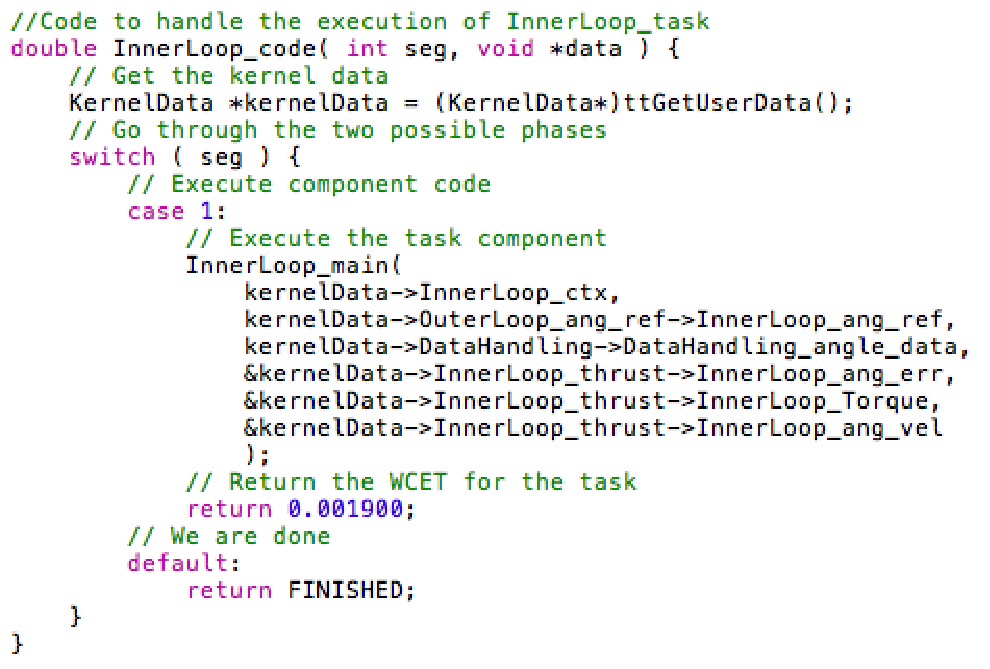
\includegraphics[width=\columnwidth]{figures/task_exec.pdf}
    \caption{InnerLoop component execution code within the TrueTime model}
    \label{fig:task_exec}
\end{figure}
Fig. \ref{fig:task_exec} shows the corresponding code that is invoked when the InnerLoop component is executed.  ESMoL task executions are always contained in a single segment.  All input and output messages are implemented as generated structures contained within the user data context.  The ESMoL task simply calls to the corresponding functional code method that was generated for that task, passing in input data values and pointers to output data locations.  This approach for input and output messages adheres to the logical execution time semantics mentioned in Section 2.  The segment finishes by returning the expected worst-case execution time (WCET) for that task given in the ESMoL model.  TrueTime will always try to let the task execution continue by calling it again with a segment value of 2, but the task will signal it has completed executing by returning the TrueTime defined value FINISHED.

When our scheduler finds no more tasks to execute in a hyperperiod it signals TrueTime that it has completed execution by returning FINISHED.  This cycle is repeated each hyperperiod until the overall simulation is halted.  TrueTime provides output ports on each kernel block that chart the execution states of all tasks.  Fig. \ref{fig:rs_schedule} shows one hyperperiod of execution for the RS node.
\begin{figure}[ht]
\centering
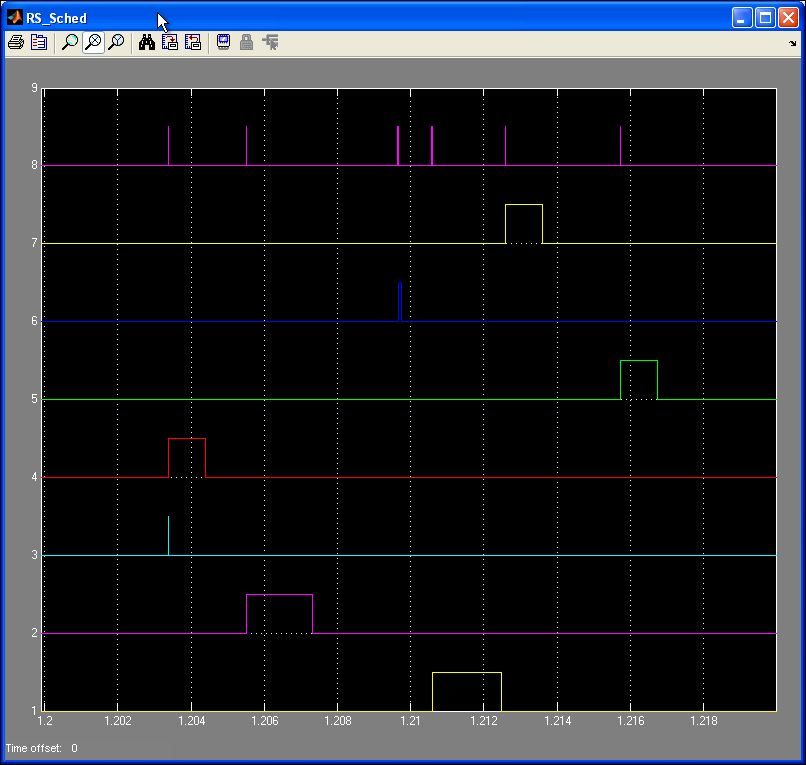
\includegraphics[width=\columnwidth]{figures/rs_schedule.jpg}
    \caption{A single hyperperiod of the task execution schedule for the RS node}
    \label{fig:rs_schedule}
\end{figure}
The top line in the chart is the ESMoL scheduler while all lines below it are individual ESMoL tasks.  For our example there are seven tasks that are executed on the RS node every hyperperiod.  One each for the DataHandler and InnerLoop components.  One for each analog input, ADC and SerialIn, and output, SerialOut.  Finally, there is also a separate task for each message sent or received over the network.  In this case, one message is sent from the RS node to the GS node and one received back.  This ensures that all network communications remain accurate to the TTA semantics.

The purpose of the TrueTime model is to allow designers to simulate and analyze deployment platform induced effects on their controllers.  Fig. \ref{fig:quadintegrator_results}(a) shows the position output of the time-invariant Simulink model compared to the synthesized TrueTime model, and (b) shows the thrust commands (top) and TrueTime model error (bottom).
\begin{figure}[t]
\centering
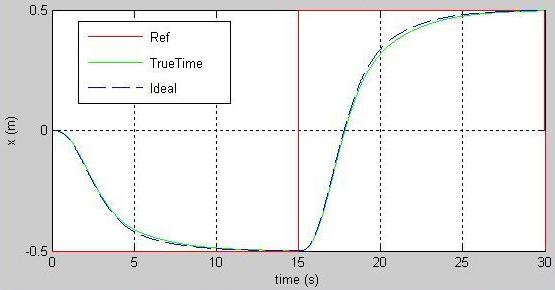
\includegraphics[width=\columnwidth]{figures/results.jpg}
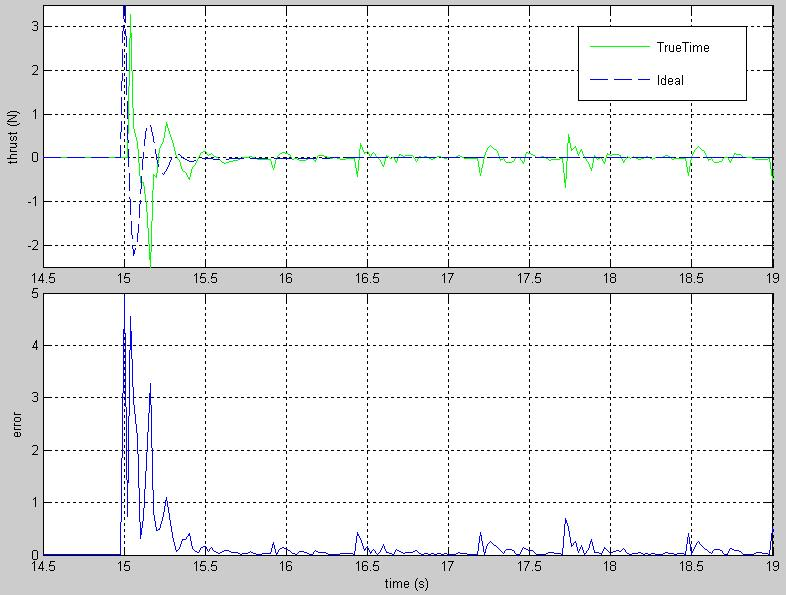
\includegraphics[width=\columnwidth]{figures/results2.jpg}
    \caption{(a) Position tracking (b) Thrust command comparison and (c) TrueTime error}
    \label{fig:quadintegrator_results}
\end{figure}
The time-invariant Simulink model does not contain any delays between the DataHandler, InnerLoop, and OuterLoop subsystems, therefore these blocks calculate output synchronously given input from the Reference signal and the plant blocks.  In contrast, the TrueTime model has propagation delays introduced by the deployment of its components onto hardware and the communications between components.  The schedule causes a total of two hyperperiods to elapse between an input and its associated output response.  The TrueTime model tracks position well, but does introduce nominal variance in the thrust output.  From the tracking we see that this variance does not destabilize the system.
